\textit{Gobuster}\cite{gobuster} es una herramienta escrita en \textit{Golang} utilizada para realizar fuerza bruta en \acrshort{uri}s, en \acrshort{dns}, en servidores web y en \textit{buckets} de \textit{Amazon S3}.\\

\textit{Gobuster} destaca por tener varios modos de escaneo.

\begin{itemize}
    \item Modo \texttt{\textbf{dir}}: el modo clásico de escaneo de directorios mediante fuerza bruta.
    \item Modo \texttt{\textbf{dns}}: modo de fuerza bruta mediante subdominios \acrshort{dns}.
    \item Modo \texttt{\textbf{fuzz}}: utilizado para hacer \textit{fuzzing}.
    \item Modo \texttt{\textbf{s3}}: enumera \textit{buckets S3} abiertos y mira por la existencia de listados de \textit{buckets}.
    \item Modo \texttt{\textbf{vhost}}: fuerza bruta mediante hosts virtuales.
\end{itemize}

\textit{Gobuster} tiene varias opciones para su uso, como se muestra en la figura \ref{fig:gobuster-help}, además de aún más opciones dependiendo del modo de uso elegido.

\begin{figure}[h]
    \centering
    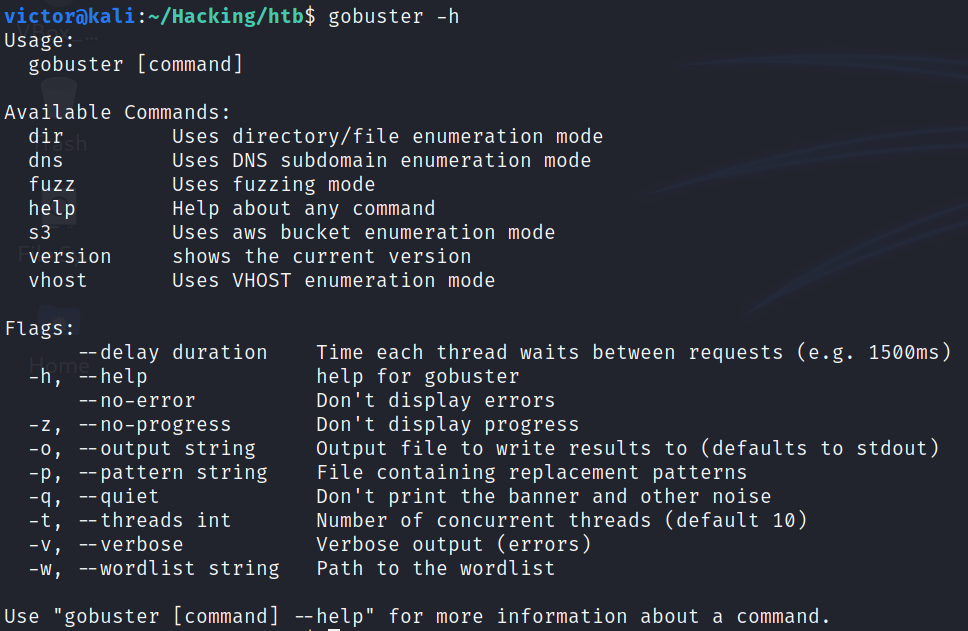
\includegraphics[width=0.7\textwidth]{images/sections/tools/gobuster.png}
    \caption{Ayuda de general de \textit{Gobuster}}
    \label{fig:gobuster-help}
\end{figure}

Algunos ejemplos de su uso son:

\begin{lstlisting}[language=bash]
gobuster dir -u https://mysite.com/path/to/folder -c 'session=123456' -t 50 -w common-files.txt -x .php,.html
gobuster dns -d mysite.com -t 50 -w common-names.txt
gobuster fuzz -u https://example.com?FUZZ=test -w parameter-names.txt
\end{lstlisting}